% MTL730 -- Lectures 1 and 9 through 12
\documentclass[11pt]{article}

\usepackage[a4paper,margin=1in]{geometry}
\usepackage{amsmath,amssymb,amsthm,mathtools}
\usepackage{enumitem}
\usepackage{graphicx}
\usepackage{array}
\usepackage{float}
\usepackage{setspace}
\usepackage{tikz}
\usepackage{microtype}
\usepackage{hyperref}

\hypersetup{
    colorlinks=true,
    linkcolor=blue,
    urlcolor=blue,
    citecolor=blue
}

\setstretch{1.17}
\setlength{\parskip}{0.55em plus 0.15em minus 0.08em}
\setlength{\parindent}{1.2em}
\setlength{\abovedisplayskip}{12pt plus 4pt minus 6pt}
\setlength{\belowdisplayskip}{12pt plus 4pt minus 6pt}
\setlength{\abovedisplayshortskip}{8pt plus 3pt}
\setlength{\belowdisplayshortskip}{8pt plus 3pt}
\setlength{\floatsep}{14pt plus 4pt minus 4pt}
\setlength{\textfloatsep}{16pt plus 4pt minus 4pt}
\setlength{\intextsep}{14pt plus 4pt minus 3pt}

\setlist{topsep=0.55em, partopsep=0.2em, itemsep=0.38em, parsep=0.12em}

\makeatletter
\renewcommand{\section}{\@startsection{section}{1}{\z@}%
    {-4.4ex \@plus -1.2ex \@minus -.2ex}%
    {2.6ex \@plus .35ex}%
    {\normalfont\Large\bfseries}}
\renewcommand{\subsection}{\@startsection{subsection}{2}{\z@}%
    {-3.5ex \@plus -1ex \@minus -.2ex}%
    {1.8ex \@plus .25ex}%
    {\normalfont\large\bfseries}}
\def\thm@space@setup{%
    \thm@preskip=0.95em plus 0.35em minus 0.2em
    \thm@postskip=0.95em plus 0.35em minus 0.2em
}
\makeatother

\setcounter{tocdepth}{2}

\newcommand{\lectureheading}[1]{%
    \clearpage
    \phantomsection
    \addcontentsline{toc}{part}{#1}%
    \section*{#1}
    \vspace{0.35em}%
}

\newtheorem{theorem}{Theorem}[section]
\newtheorem{lemma}[theorem]{Lemma}
\newtheorem{proposition}[theorem]{Proposition}
\newtheorem{corollary}[theorem]{Corollary}
\newtheorem{definition}[theorem]{Definition}
\newtheorem{example}[theorem]{Example}
\newtheorem{claim}[theorem]{Claim}
\theoremstyle{remark}
\newtheorem*{remark}{Remark}

\makeatletter
\def\thm@space@setup{%
    \thm@preskip=0.95em plus 0.35em minus 0.2em
    \thm@postskip=0.95em plus 0.35em minus 0.2em
}
\makeatother

\DeclareMathOperator{\gcdop}{gcd}
\DeclareMathOperator{\ord}{ord}
\DeclareMathOperator{\ind}{ind}
\newcommand{\Z}{\mathbb Z}
\newcommand{\N}{\mathbb N}
\newcommand{\R}{\mathbb R}
\newcommand{\Fp}{\mathbb F_p}
\newcommand{\units}[1]{\left(\mathbb Z/#1\mathbb Z\right)^\times}

\title{\textbf{MTL730 --- Lectures 1 and 9--12}\\[2mm]
\large Classical Ciphers, Complexity, and Public-Key Cryptography}
\author{}
\date{}

\begin{document}
\maketitle
\begingroup
\setlength{\parskip}{0.12em plus 0.05em}
\setstretch{1.08}
\tableofcontents
\endgroup
\newpage

\lectureheading{Lecture 1}

% ============================================================
\section{Monoalphabetic Substitution}
% ============================================================

Throughout these lectures, letters are encrypted independently of word
boundaries: spaces may be kept for readability, but they are not part of
the mathematical key. Two numbering conventions appear in the course.

\begin{itemize}[leftmargin=1.4em]
    \item \textbf{Zero-based:} $a=0,\,b=1,\,\ldots,\,z=25$. This is the
    convention used from 1 September onward (Hill, autokey, modular
    arithmetic).
    \item \textbf{One-based:} $A=1,\,B=2,\,\ldots,\,Z=26$. The handwritten
    Vigen\`ere example ``today is tuesday'' was computed in this convention.
\end{itemize}
Unless stated otherwise, we work with $a=0,\ldots,z=25$ and arithmetic
modulo $26$.

\begin{definition}[Caesar cipher]
Fix a shift $k\in\{0,1,\ldots,25\}$. Encryption is the map
\[
    x \longmapsto x+k \pmod{26}.
\]
Decryption is the shift $-k$.
\end{definition}

\begin{example}
Plaintext \texttt{enemy is falling back}, shift $k=5$:
\[
\begin{array}{cccccccccccc}
\text{e n e m y} && \text{i s} && \text{f a l l i n g} && \text{b a c k}\\
\text{J S J R D} && \text{N X} && \text{K F Q Q N S L} && \text{G F H P}.
\end{array}
\]
Ciphertext: \texttt{JSJRD NX KFQQNSL GFHP}.
\end{example}

\begin{example}
Plaintext \texttt{cryptography is fun}, shift $k=3$:
\[
    \texttt{FUBSWRJUDSKB LV IXQ}.
\]
\end{example}

A Caesar cipher is determined by a single parameter, so it is broken as
soon as one plaintext--ciphertext pair of letters is guessed. A general
monoalphabetic substitution uses an arbitrary permutation of the alphabet
and therefore has
\[
    26!\approx 4.03\times 10^{26}
\]
keys. Exhaustive search is impossible, but English is highly non-uniform,
so frequency analysis still recovers the permutation.

\begin{figure}[H]
\centering
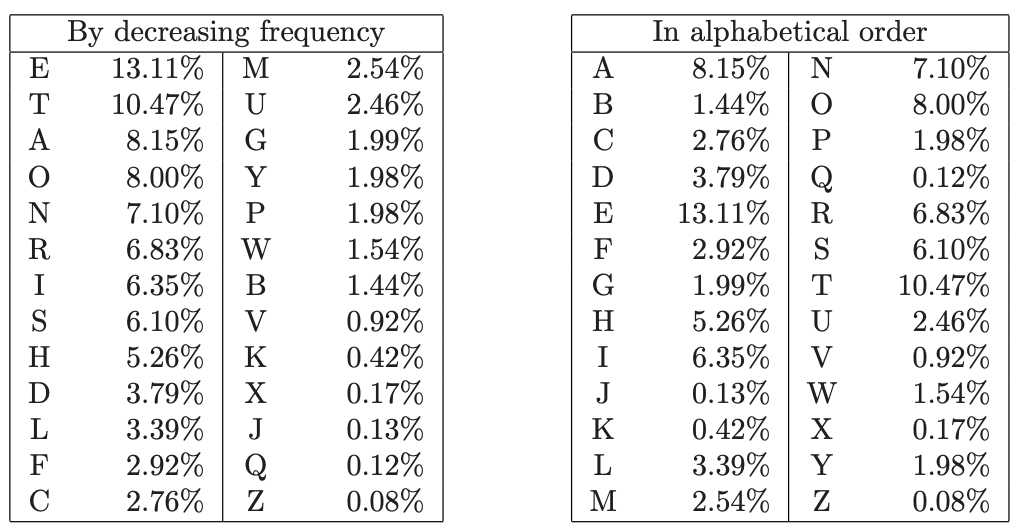
\includegraphics[width=0.98\textwidth]{figures/english_frequencies.png}
\caption{Typical English letter frequencies (from the course handout).
The five most common letters are E, T, A, O, N.}
\end{figure}

\begin{figure}[H]
\centering
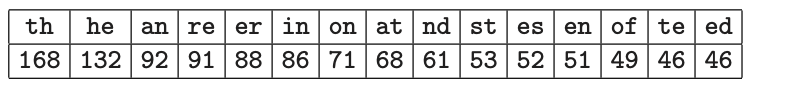
\includegraphics[width=0.95\textwidth]{figures/english_bigrams.png}
\caption{Most common English bigrams (frequency per $1000$ words).}
\end{figure}

% ------------------------------------------------------------
\subsection{Cryptanalysis by guessing common words}
% ------------------------------------------------------------

\begin{example}
Ciphertext
\[
    \texttt{ESTYRD LCP DPWOZX LD ESPJ DPPX}.
\]
The three-letter block \texttt{LCP} is a natural candidate for
\texttt{are}. That single guess forces the shift
\[
    \texttt{a}\mapsto\texttt{L},
\]
hence $k=11$, and the plaintext is
\[
    \texttt{things are seldom as they seem}.
\]
\end{example}

\begin{example}[Mixed alphabet]
An arbitrary permutation in five-letter groups, as in the handout
(each plaintext letter sits directly above its ciphertext letter):
\begin{center}
\resizebox{\linewidth}{!}{%
\ttfamily\setlength{\tabcolsep}{3.2pt}%
\begin{tabular}{@{}*{5}{c}@{\hspace{0.9em}}*{5}{c}@{\hspace{0.9em}}*{5}{c}@{\hspace{0.9em}}*{5}{c}@{\hspace{0.9em}}*{5}{c}@{\hspace{0.9em}}c@{}}
a&b&c&d&e&f&g&h&i&j&k&l&m&n&o&p&q&r&s&t&u&v&w&x&y&z\\
X&H&Z&R&W&F&G&P&T&Y&J&O&C&A&E&U&L&N&K&Q&I&V&S&M&D&B
\end{tabular}}
\end{center}
Under this key,
\[
    \texttt{cryptography is fun}
    \longmapsto
    \texttt{ZNDUQEGNXUPD TK FIA}.
\]
The inverse substitution (ciphertext letter $\mapsto$ plaintext letter) is
\begin{center}
\resizebox{\linewidth}{!}{%
\ttfamily\setlength{\tabcolsep}{3.2pt}%
\begin{tabular}{@{}*{5}{c}@{\hspace{0.9em}}*{5}{c}@{\hspace{0.9em}}*{5}{c}@{\hspace{0.9em}}*{5}{c}@{\hspace{0.9em}}*{5}{c}@{\hspace{0.9em}}c@{}}
A&B&C&D&E&F&G&H&I&J&K&L&M&N&O&P&Q&R&S&T&U&V&W&X&Y&Z\\
n&z&m&y&o&f&g&b&u&k&s&q&x&r&l&h&t&d&w&i&p&v&e&a&j&c
\end{tabular}}
\end{center}
\end{example}

\begin{example}
Ciphertext \texttt{T SXAQ X LITZJ LIWKQTEA} decrypts, by successive
guesses that exploit short words and repeated fragments, as follows.
\[
\begin{array}{ll}
\text{ciphertext} & \texttt{T SXAQ X LITZJ LIWKQTEA}\\
\text{guess \texttt{i}/\texttt{a}} &
\texttt{i SaAQ a LIiZJ LIWKQiEA}\\
\text{guess \texttt{qui}} &
\texttt{i SaAQ a quiZJ quWKQiEA}\\
\text{guess \texttt{quick}} &
\texttt{i SaAQ a quick quWKQiEA}\\
\text{guess \texttt{question}} &
\texttt{i Sant a quick question}\\
\text{plaintext} &
\texttt{i want a quick question}.
\end{array}
\]
\end{example}

% ------------------------------------------------------------
\subsection{A longer substitution: frequency, bigrams, and cribs}
% ------------------------------------------------------------

\begin{example}[Sherlock Holmes passage]
The ciphertext (written in five-letter groups) is
{\footnotesize
\begin{align*}
&\texttt{LOJUM YLJME PDYVJ QXTDV SVJNL DMTJZ WMJGG YSNDL UYLEO SKDVC}\\
&\texttt{GEPJS MDIPD NEJSK DNJTJ LSKDL OSVDV DNGYN VSGLL OSCIO LGOYG}\\
&\texttt{ESNEP CGYSN GUJMJ DGYNK DPPYX PJDGG SVDNT WMSWS GYLYS NGSKJ}\\
&\texttt{CEPYQ GSGLD MLPYN IUSCP QOYGM JGCPL GDWWJ DMLSL OJCNY NYLYD}\\
&\texttt{LJQLO DLCNL YPLOJ TPJDM NJQLO JWMSE JGGJG XTUOY EOOJO DQDMM}\\
&\texttt{YBJQD LLOJV LOJTV YIOLU JPPES NGYQJ MOYVD GDNJE MSVDN EJM}.
\end{align*}
}

\begin{figure}[H]
\centering
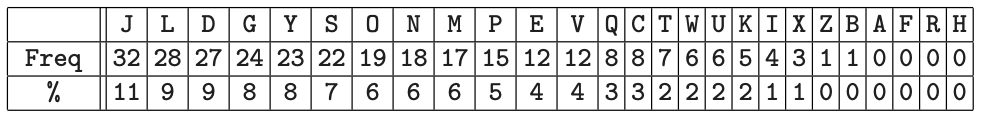
\includegraphics[width=0.98\textwidth]{figures/ex6_cipher_freq.png}
\caption{Letter counts in the ciphertext. \texttt{J} is the most frequent
symbol, so it is the first candidate for plaintext \texttt{e}.}
\end{figure}

\begin{figure}[H]
\centering
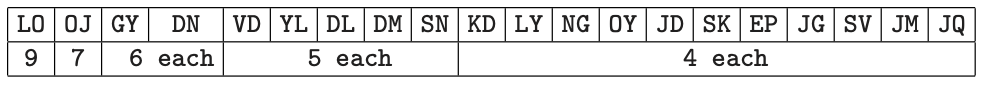
\includegraphics[width=0.92\textwidth]{figures/ex6_cipher_bigrams.png}
\caption{Repeated ciphertext bigrams. High-frequency English bigrams such
as \texttt{th}, \texttt{he}, \texttt{in}, \texttt{an} are the natural
cribs.}
\end{figure}

\begin{figure}[H]
\centering
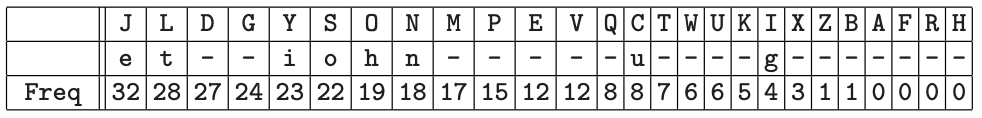
\includegraphics[width=0.98\textwidth]{figures/ex6_partial_map.png}
\caption{Partial substitution obtained from frequencies: \texttt{J}$\mapsto$e,
\texttt{L}$\mapsto$t, and so on.}
\end{figure}

A typical reconstruction, as in the handout, proceeds by cribs rather
than by brute force.
\begin{itemize}[leftmargin=1.4em]
    \item \texttt{J} is the most frequent ciphertext letter, hence
    \texttt{e}.
    \item The block \texttt{VSGLL OSCIO LGOYG} contains
    \texttt{---tt h---h t-h--}. The English word \texttt{thought} forces
    \texttt{SCI}$\mapsto$\texttt{oug}.
    \item \texttt{YIOLU} as \texttt{-ght-} forces \texttt{Y}$\mapsto$\texttt{i}.
    \item \texttt{GYLYSN} as \texttt{-ition} forces \texttt{sition}, hence
    \texttt{N}$\mapsto$\texttt{n} and then \texttt{G}$\mapsto$\texttt{s}.
    \item \texttt{DLCNL YPLOJ} as \texttt{atunt i-the} is
    \texttt{at until the}, so \texttt{P}$\mapsto$\texttt{l}.
    \item \texttt{WMSWS GYLYS NGSKJ} becomes \texttt{propo sition}, so
    \texttt{W}$\mapsto$\texttt{p} and \texttt{M}$\mapsto$\texttt{r}.
    \item Continuing in this way yields \texttt{Z}$\mapsto$\texttt{x},
    \texttt{E}$\mapsto$\texttt{c}, \texttt{Q}$\mapsto$\texttt{d},
    \texttt{V}$\mapsto$\texttt{m}, \texttt{U}$\mapsto$\texttt{w}.
\end{itemize}
The plaintext is the Holmes description of deduction from
\emph{A Study in Scarlet}:
\begin{quote}
The writer claimed by a momentary expression, a twitch of a muscle or a
glance of an eye, to fathom a man's inmost thoughts. His conclusions were
as infallible as so many propositions of Euclid. So startling would his
results appear to the uninitiated that until they learned the processes
by which he had arrived at them they might well consider him as a
necromancer.
\end{quote}
\end{example}

Monoalphabetic ciphers preserve the non-uniformity of English, which is
why the attack works. Polyalphabetic ciphers, introduced next, try to
flatten those frequencies by using several Caesar alphabets in rotation.

\lectureheading{Lecture 9}

% ============================================================
\section{The Vigen\`ere Cipher}
% ============================================================

\begin{definition}[Vigen\`ere cipher]
Let the key be a word $k=k_0k_1\cdots k_{\ell-1}$ of length $\ell$.
Writing letters as integers modulo $26$, the $i$-th plaintext letter
$p_i$ is encrypted by
\[
    c_i \equiv p_i + k_{i \bmod \ell} \pmod{26}.
\]
Equivalently, one looks up $p_i$ in the Vigen\`ere square in the row
indexed by the current key letter.
\end{definition}

The cipher is \emph{polyalphabetic}: there are $\ell$ distinct Caesar
alphabets, reused periodically.

\begin{figure}[H]
\centering
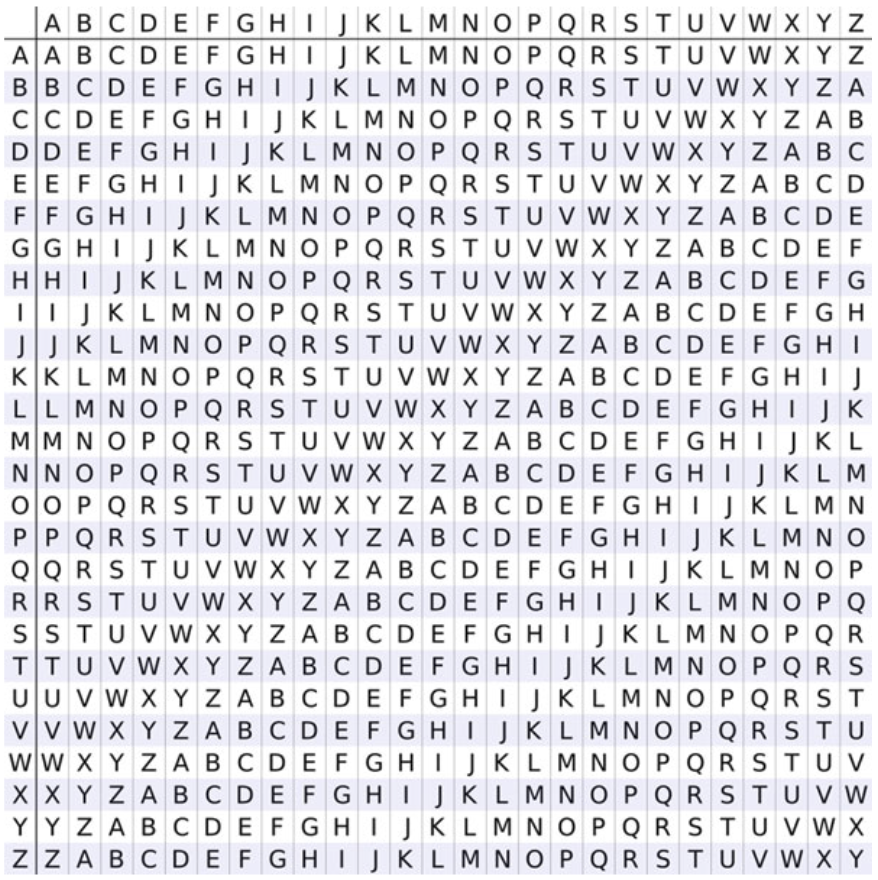
\includegraphics[width=\linewidth]{figures/vigenere_square.png}
\caption{The Vigen\`ere square. The row is the key letter and the column
is the plaintext letter; their intersection is the ciphertext letter
(zero-based convention).}
\end{figure}

\begin{example}[Handwritten lecture: one-based arithmetic]
Plaintext \texttt{today is tuesday}, key \texttt{HARD} repeated:
\[
\begin{array}{l}
\texttt{t o d a y i s t u e s d a y}\\
\texttt{H A R D H A R D H A R D H A}\\
\texttt{B P V E G J K X C F K H I Z}.
\end{array}
\]
Here $A=1,\ldots,Z=26$, so for instance
\[
    \texttt{t}=20,\quad \texttt{H}=8,\quad
    20+8=28\equiv 2 \pmod{26}
\]
which is \texttt{B}, and the tenth letter is
\[
    \texttt{e}=5,\quad \texttt{A}=1,\quad 5+1=6 \mapsto \texttt{F}.
\]
Grouped with the original spacing:
\[
    \texttt{BPVEG JK XCFKHIZ}.
\]
(The notebook wrote \texttt{XCTKHIZ}; the \texttt{T} is a slip for
\texttt{F}.)
\end{example}

\begin{example}[Course handout, 29 August, zero-based]
Plaintext \texttt{this is saturday morning}. The keystream written in
the handout is
\[
    \texttt{RAKH IR AKHIRAKH IRAKHIR},
\]
which is the $5$-letter keyword \texttt{RAKHI} repeated (not
\texttt{RAKHIR}):
\[
\begin{array}{l}
\texttt{t h i s i s s a t u r d a y m o r n i n g}\\
\texttt{R A K H I R A K H I R A K H I R A K H I R}\\
\texttt{K H S Z Q J S K A C I D K F U F R X P V X}.
\end{array}
\]
Check the first letter in the $a=0$ convention:
\[
    \texttt{t}=19,\quad \texttt{R}=17,\quad
    19+17=36\equiv 10 \pmod{26},
\]
which is \texttt{K}. Ciphertext: \texttt{KHSZ QJ SKACIDKF UFRXPVX}.
\end{example}

% ------------------------------------------------------------
\subsection{Kasiski examination}
% ------------------------------------------------------------

\begin{definition}[Kasiski examination]
Repeated fragments in a Vigen\`ere ciphertext usually come from the same
plaintext fragment encrypted with the same key alignment. Therefore the
distance between two occurrences of a repeated string is a multiple of
the key length $\ell$. The greatest common divisor of several such
distances is a multiple of $\ell$ --- equivalently, $\ell$ divides that
gcd --- and often the gcd equals $\ell$.
\end{definition}

The attack has two stages: guess $\ell$, then recover each of the $\ell$
Caesar alphabets by ordinary frequency analysis.

\begin{example}
If a fragment \texttt{tion} occurs twice, encrypted once under
\texttt{HARD} and once under the same four letters later, the distance
between the two occurrences is a multiple of $4$. The same holds for a
repeated \texttt{ture} aligned under \texttt{RDHA}.
\end{example}

\begin{example}[Lobachevsky ciphertext]
A long Vigen\`ere ciphertext from the handout (Tom Lehrer's
\emph{Lobachevsky}) begins
{\footnotesize
\begin{align*}
&\texttt{OWWPE UWBMW LVYTV LYJAP UWSUS NBKID SIPHQ RLXKL}\\
&\texttt{EELWI WSKZT ZVECD FCRXV OWWVX YWEZR JVKHW UXYSI}\\
&\texttt{UDHVE TBKEK OPGWL VYGMD XVKIB KEKWK MUKFL RPDPB}\quad\cdots
\end{align*}
}
Repeated strings and the distances between their first and second
occurrences are recorded below.

\begin{figure}[H]
\centering
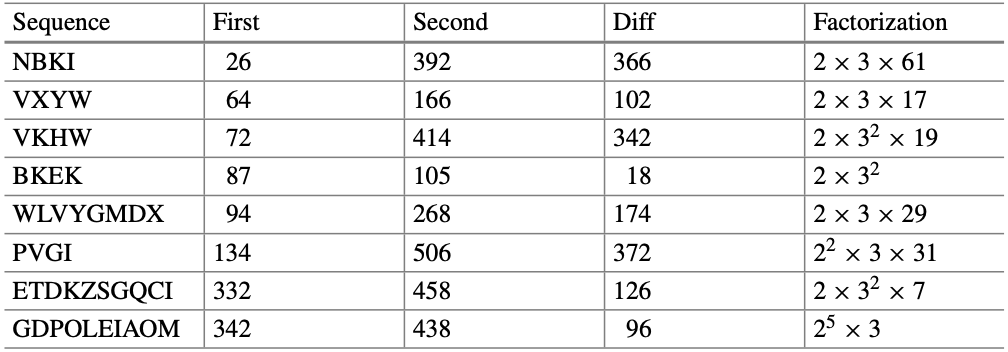
\includegraphics[width=0.98\textwidth]{figures/kasiski_repeats.png}
\caption{Kasiski distances in the Lobachevsky ciphertext. The gcd of the
listed differences is $6$, so $\ell$ divides $6$. Combined with Friedman
and column indices of coincidence, one takes $\ell=6$.}
\end{figure}

The plaintext, recovered once the key length is known, is Lehrer's lyric
beginning ``Who made me the genius I am today, the mathematician that
others all quote? \ldots Nicolai Ivanovich Lobachevsky is his name.''
\end{example}

% ------------------------------------------------------------
\subsection{Friedman test: the index of coincidence}
% ------------------------------------------------------------

\begin{definition}[Index of coincidence]
Let a text of length $N$ contain the $i$-th letter of the alphabet $f_i$
times, for $i=0,\ldots,25$. The index of coincidence is
\[
    I_C
    =
    \frac{\displaystyle\sum_{i=0}^{25} f_i(f_i-1)}{N(N-1)}.
\]
It is the probability that two distinct positions, drawn uniformly
without replacement, carry the same letter.
\end{definition}

For English plaintext one has
\[
    I_E \approx \sum_{i=0}^{25} p_i^2 \approx 0.0667,
\]
where $p_i$ are the English letter probabilities. For a uniformly random
string over $26$ letters,
\[
    I_R = \frac1{26}\approx 0.0385.
\]
A monoalphabetic ciphertext still has $I_C\approx I_E$. A Vigen\`ere
ciphertext with a long key looks more random, so $I_C$ drops toward
$I_R$.

Now fix a candidate key length $\ell$ and put the ciphertext into $\ell$
baskets according to position modulo $\ell$. Two randomly chosen letters
then fall into one of two events.

\begin{itemize}[leftmargin=1.4em]
    \item They lie in the \emph{same} basket (probability about
    $1/\ell$). That basket is a Caesar ciphertext of English, so the
    coincidence probability is about $I_E$.
    \item They lie in \emph{different} baskets (probability about
    $(\ell-1)/\ell$). If the corresponding key letters behave like
    independent shifts, the coincidence probability is about $I_R$.
    (A keyword with repeated letters makes this only approximate.)
\end{itemize}
Hence
\[
    I_C
    \;\approx\;
    \frac1\ell\, I_E
    +
    \frac{\ell-1}{\ell}\, I_R
    =
    I_R + \frac1\ell\,(I_E-I_R).
\]
Solving for the key length gives Friedman's estimate
\[
    \ell
    \;\approx\;
    \frac{I_E-I_R}{I_C-I_R}.
\]

\begin{remark}
The formula is only an approximation, and it fails for ciphers whose key
does not repeat a fixed alphabet (autokey, running-key, one-time pad).
Even for genuine Vigen\`ere, a non-integral estimate such as
$\ell\approx 7.57$ must be checked against nearby candidate lengths
($6$, $7$, $8$, \ldots) by computing the index of coincidence of each
column. For the Lobachevsky ciphertext one finds $I_C\approx 0.0425$, so
Friedman suggests $\ell\approx 7$; Kasiski gives $\ell\mid 6$; and the
six columns for $\ell=6$ each have $I_C$ near $I_E$, which confirms the
key length.
\end{remark}

\begin{figure}[H]
\centering
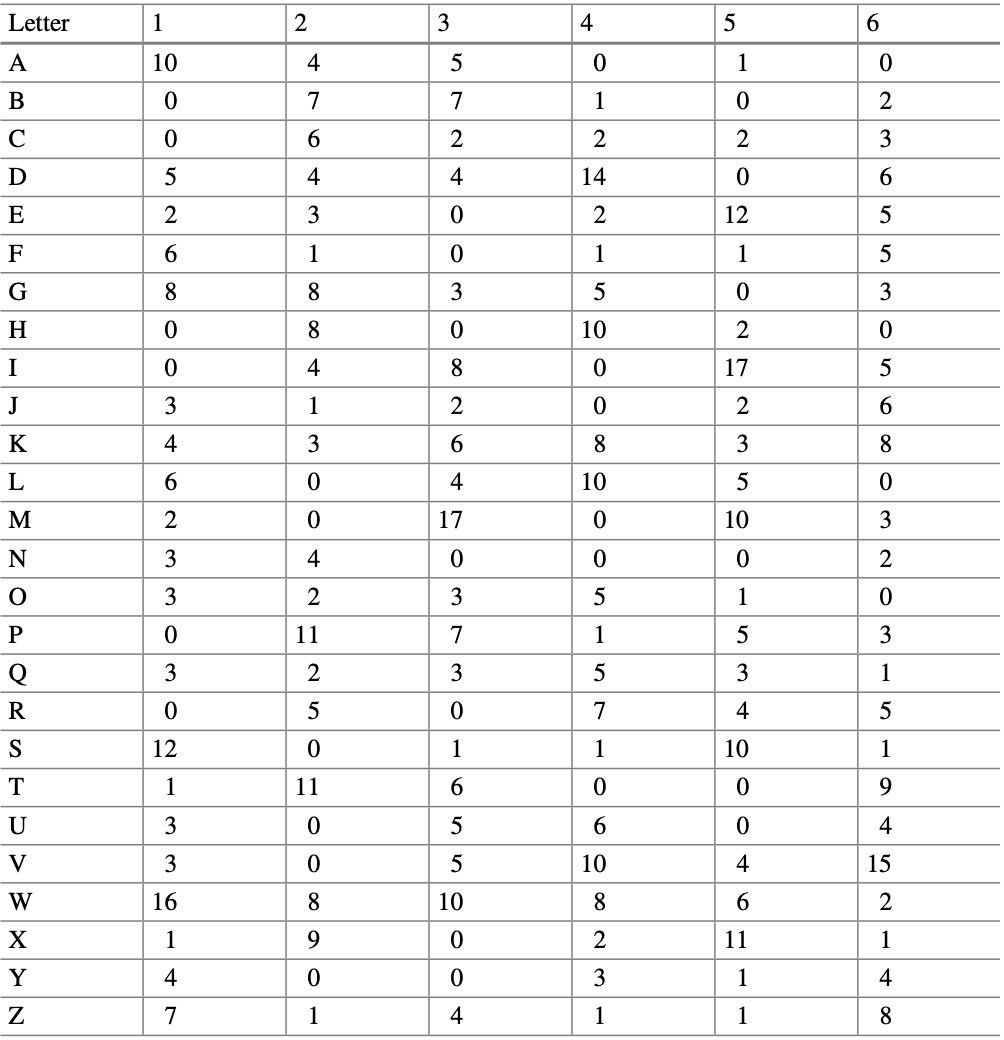
\includegraphics[width=\linewidth]{figures/friedman_columns.png}
\caption{Letter counts in the six residue classes modulo $\ell=6$ for the
Lobachevsky ciphertext. Each column is a Caesar cipher and can be broken
by ordinary frequency analysis.}
\end{figure}

\lectureheading{Lecture 10}

% ============================================================
\section{Autokey Cipher}
% ============================================================

\begin{definition}[Autokey]
Choose a primer key $k_0k_1\cdots k_{m-1}$. Encrypt the first $m$
plaintext letters as in Vigen\`ere. Thereafter the key stream is the
plaintext itself:
\[
    k_{m+i}=p_i.
\]
In other words, once the primer is exhausted one uses the message as its
own key.
\end{definition}

Kasiski and Friedman both rely on a \emph{periodic} key, so they do not
apply directly to autokey.

\begin{example}[1 September]
Plaintext: \texttt{this is to learn autokey cipher}.\\
Primer: \texttt{DEMONSTRATION}, after which the plaintext is recycled as key:
\[
\begin{array}{l}
\texttt{t h i s i s t o l e a r n a u t o k e y c i p h e r}\\
\texttt{D E M O N S T R A T I O N T H I S I S T O L E A R N}\\
\texttt{W L U G V K M F L X I F A T B B G S W R Q T T H V E}.
\end{array}
\]
The first letter in the $a=0$ convention:
\[
    \texttt{t}=19,\quad \texttt{D}=3,\quad 19+3=22 \mapsto \texttt{W}.
\]
Ciphertext: \texttt{WLUG VK MF LXIFA TBBGSWR QTTHVE}.
\end{example}

% ============================================================
\section{Hill Cipher}
% ============================================================

\begin{definition}[Hill cipher]
Fix an integer block length $n\ge 2$ and an invertible matrix
$A\in\mathrm{M}_n(\Z/26\Z)$, that is
\[
    \gcdop(\det A,\,26)=1.
\]
Plaintext is written as column vectors of length $n$ with $a=0,\ldots,z=25$.
Encryption of a block $p$ is
\[
    c \equiv A p \pmod{26}.
\]
Decryption is multiplication by $A^{-1}$.
\end{definition}

If the last block is short, one pads (the lecture used \texttt{z}).

\begin{example}[$n=3$]
Take
\[
    A
    =
    \begin{pmatrix}
    1 & 2 & 3 \\
    2 & 3 & 6 \\
    3 & 6 & 18
    \end{pmatrix}.
\]
Then
\[
    \det A = -9 \equiv 17 \pmod{26},
    \qquad
    \gcdop(17,26)=1,
\]
so $A$ is invertible modulo $26$. The inverse, which is needed for
decryption, is
\[
    A^{-1}
    \equiv
    \begin{pmatrix}
    24 & 2 & 17 \\
    2 & 25 & 0 \\
    17 & 0 & 3
    \end{pmatrix}
    \pmod{26}.
\]
Plaintext \texttt{this is to learn hill cipher}, grouped in threes and
padded, is
\[
    \texttt{thi sis tol ear nhi llc iph erz}.
\]
The first three blocks are
\begin{align*}
    A
    \begin{pmatrix} 19 \\ 7 \\ 8 \end{pmatrix}
    &\equiv
    \begin{pmatrix} 5 \\ 3 \\ 9 \end{pmatrix}
    \pmod{26}
    &&\texttt{thi}\mapsto\texttt{fdj},\\[4pt]
    A
    \begin{pmatrix} 18 \\ 8 \\ 18 \end{pmatrix}
    &\equiv
    \begin{pmatrix} 10 \\ 12 \\ 10 \end{pmatrix}
    \pmod{26}
    &&\texttt{sis}\mapsto\texttt{kmk},\\[4pt]
    A
    \begin{pmatrix} 19 \\ 14 \\ 11 \end{pmatrix}
    &\equiv
    \begin{pmatrix} 2 \\ 16 \\ 1 \end{pmatrix}
    \pmod{26}
    &&\texttt{tol}\mapsto\texttt{cqb}.
\end{align*}
Continuing through the remaining blocks gives the ciphertext
\[
    \texttt{fdj kmk cqb dgg zrr npf hzg jbs}.
\]
(The typed handout listed the first block as \texttt{bdj}; that is the
slip $57\equiv 1\pmod{26}$ instead of $57\equiv 5$. The second component
$107\equiv 3$ and the third $243\equiv 9$ are correct, and the second
block \texttt{kmk} matches.)
\end{example}

% ------------------------------------------------------------
\subsection{\texorpdfstring{Known-plaintext attack on a $2\times 2$ Hill cipher}{Known-plaintext attack on a 2x2 Hill cipher}}
% ------------------------------------------------------------

If $n$ linearly independent plaintext blocks and their ciphertexts are
known, the key matrix is recovered by linear algebra over $\Z/26\Z$.

\begin{example}
Suppose $n=2$ and
\[
    \texttt{th}\mapsto\texttt{BP},
    \qquad
    \texttt{he}\mapsto\texttt{CX}.
\]
In numbers,
\[
    A
    \begin{pmatrix} 19 \\ 7 \end{pmatrix}
    \equiv
    \begin{pmatrix} 1 \\ 15 \end{pmatrix},
    \qquad
    A
    \begin{pmatrix} 7 \\ 4 \end{pmatrix}
    \equiv
    \begin{pmatrix} 2 \\ 23 \end{pmatrix}
    \pmod{26},
\]
or, as a single matrix equation,
\[
    A
    \begin{pmatrix}
    19 & 7 \\
    7 & 4
    \end{pmatrix}
    \equiv
    \begin{pmatrix}
    1 & 2 \\
    15 & 23
    \end{pmatrix}
    \pmod{26}.
\]
The plaintext matrix has determinant
\[
    19\cdot 4 - 7\cdot 7 = 76-49=27\equiv 1 \pmod{26},
\]
so it is invertible, with inverse
\[
    \begin{pmatrix}
    19 & 7 \\
    7 & 4
    \end{pmatrix}^{-1}
    \equiv
    \begin{pmatrix}
    4 & 19 \\
    19 & 19
    \end{pmatrix}
    \pmod{26}
\]
(the cofactor matrix of a determinant-$1$ matrix, reduced modulo $26$,
using $-7\equiv 19$). Therefore
\begin{align*}
    A
    &\equiv
    \begin{pmatrix} 1 & 2 \\ 15 & 23 \end{pmatrix}
    \begin{pmatrix} 4 & 19 \\ 19 & 19 \end{pmatrix}
    \equiv
    \begin{pmatrix} 16 & 5 \\ 3 & 20 \end{pmatrix}
    \pmod{26}.
\end{align*}
The key has been recovered from four known letters.
\end{example}

% ============================================================
\section{Transposition Ciphers}
% ============================================================

Substitution ciphers permute the \emph{alphabet}. Transposition ciphers
permute the \emph{positions} of the letters.

% ------------------------------------------------------------
\subsection{Rail fence}
% ------------------------------------------------------------

\begin{definition}[Rail fence]
The key is the number $r$ of rails. Write the plaintext along a zigzag
with $r$ rows, then read row by row.
\end{definition}

\begin{example}
Plaintext \texttt{the key is under the mat} (spaces deleted:
\texttt{thekeyisunderthemat}), key $r=4$. The letters run down to rail
$4$ and back up, one column per letter:
\begin{center}
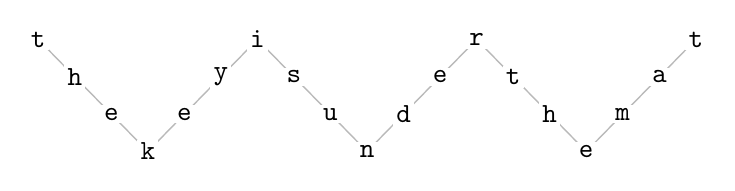
\begin{tikzpicture}[x=1.32em, y=-1.35em]
    \draw[gray!55, line width=0.5pt]
        (0,0) -- (1,1) -- (2,2) -- (3,3) -- (4,2) -- (5,1) -- (6,0)
        -- (7,1) -- (8,2) -- (9,3) -- (10,2) -- (11,1) -- (12,0)
        -- (13,1) -- (14,2) -- (15,3) -- (16,2) -- (17,1) -- (18,0);
    \foreach \x/\y/\ch in {
        0/0/t, 1/1/h, 2/2/e, 3/3/k, 4/2/e, 5/1/y, 6/0/i,
        7/1/s, 8/2/u, 9/3/n, 10/2/d, 11/1/e, 12/0/r,
        13/1/t, 14/2/h, 15/3/e, 16/2/m, 17/1/a, 18/0/t
    } {
        \node[font=\ttfamily\bfseries, fill=white, inner sep=1.2pt]
            at (\x,\y) {\ch};
    }
\end{tikzpicture}
\end{center}
Reading the four rails left to right gives
\[
    \texttt{TIRT HYSETA EEUDHM KNE}
    =
    \texttt{TIRTHYSETAEEUDHMKNE}.
\]
(The typed notes grouped this as \texttt{TIRTH YESTA EEUDH MKNE}, which
is the same string except for a transposition of \texttt{S} and
\texttt{E} in the second group.) Decryption writes the ciphertext back
into the same zigzag shape.
\end{example}

The key space is small: extra rails beyond the message length do not add
new permutations. Rail fence is therefore only a building block, not a
cipher by itself.

% ------------------------------------------------------------
\subsection{Columnar transposition}
% ------------------------------------------------------------

\begin{definition}[Columnar transposition]
Write the plaintext in rows under a keyword. Reorder the columns so that
the keyword is in alphabetical order, then read down the columns. (If the keyword has repeated letters, break
ties by left-to-right order in the keyword.)
\end{definition}

\begin{example}
Plaintext \texttt{thekeyisunderthemat}, padded with \texttt{z} to fill
the rectangle, keyword \texttt{MANGO}:
\begin{center}
\renewcommand{\arraystretch}{1.2}
\begin{tabular}{@{}c@{\qquad}c@{\qquad}c@{}}
\begin{tabular}{|c|c|c|c|c|}
\hline
M & A & N & G & O \\
\hline
T & H & E & K & E \\
Y & I & S & U & N \\
D & E & R & T & H \\
E & M & A & T & Z \\
\hline
\end{tabular}
&
$\longrightarrow$
&
\begin{tabular}{|c|c|c|c|c|}
\hline
A & G & M & N & O \\
\hline
H & K & T & E & E \\
I & U & Y & S & N \\
E & T & D & R & H \\
M & T & E & A & Z \\
\hline
\end{tabular}
\end{tabular}
\end{center}
because the alphabetical order of \texttt{MANGO} is
\texttt{A},\,\texttt{G},\,\texttt{M},\,\texttt{N},\,\texttt{O}.
Reading column by column:
\[
    \texttt{HIEMK UTTTY DEESR AENHZ}.
\]
\end{example}

% ============================================================
\section{Field Ciphers}
% ============================================================

% ------------------------------------------------------------
\subsection{ADFGX}
% ------------------------------------------------------------

The letters \texttt{A}, \texttt{D}, \texttt{F}, \texttt{G}, \texttt{X}
were chosen because they have sharply distinct Morse codes. The cipher
has two keys: a $5\times 5$ Polybius square (with \texttt{i}/\texttt{j}
identified) and a columnar transposition keyword.

\begin{example}
The handout uses a mixed $5\times 5$ square (right) in place of the
standard Polybius square (left); \texttt{i} and \texttt{j} share a cell.
\begin{center}
\renewcommand{\arraystretch}{1.15}
\begin{tabular}{@{}c@{\qquad}c@{}}
\begin{tabular}{|c||c|c|c|c|c|}
\hline
 & A & D & F & G & X \\
\hline\hline
A & a & b & c & d & e \\
\hline
D & f & g & h & i/j & k \\
\hline
F & l & m & n & o & p \\
\hline
G & q & r & s & t & u \\
\hline
X & v & w & x & y & z \\
\hline
\end{tabular}
&
\begin{tabular}{|c||c|c|c|c|c|}
\hline
 & A & D & F & G & X \\
\hline\hline
A & b & t & a & l & p \\
\hline
D & d & h & o & z & k \\
\hline
F & q & f & v & s & n \\
\hline
G & g & i/j & c & u & x \\
\hline
X & m & r & e & w & y \\
\hline
\end{tabular}\\[4pt]
\small standard & \small key 1 (lecture)
\end{tabular}
\end{center}
Plaintext \texttt{attack at once} is replaced by coordinates in the
mixed square:
\[
\begin{array}{cccccccccccc}
\texttt{a}&\texttt{t}&\texttt{t}&\texttt{a}&\texttt{c}&\texttt{k}&
\texttt{a}&\texttt{t}&\texttt{o}&\texttt{n}&\texttt{c}&\texttt{e}\\
\texttt{AF}&\texttt{AD}&\texttt{AD}&\texttt{AF}&\texttt{GF}&\texttt{DX}&
\texttt{AF}&\texttt{AD}&\texttt{DF}&\texttt{FX}&\texttt{GF}&\texttt{XF}
\end{array}
\]
The transitional string \texttt{AF AD AD AF GF DX AF AD DF FX GF XF} is
then written under the second key \texttt{CARGO} and read by columns in
alphabetical order \texttt{A}, \texttt{C}, \texttt{G}, \texttt{O},
\texttt{R}:
\begin{center}
\renewcommand{\arraystretch}{1.15}
\begin{tabular}{@{}c@{\qquad}c@{\qquad}c@{}}
\begin{tabular}{|c|c|c|c|c|}
\hline
C & A & R & G & O \\
\hline
A & F & A & D & A \\
D & A & F & G & F \\
D & X & A & F & A \\
D & D & F & F & X \\
G & F & X & F & \phantom{X} \\
\hline
\end{tabular}
&
$\longrightarrow$
&
\texttt{FAXDF ADDDG DGFFF AFAXA FAFX}
\end{tabular}
\end{center}
\end{example}

% ------------------------------------------------------------
\subsection{ADFGVX}
% ------------------------------------------------------------

The improved wartime cipher uses a $6\times 6$ square labelled
\texttt{A D F G V X}, which holds $26$ letters and $10$ digits.

\begin{example}
The square
\begin{center}
\renewcommand{\arraystretch}{1.15}
\begin{tabular}{|c||c|c|c|c|c|c|}
\hline
 & A & D & F & G & V & X \\
\hline\hline
A & n & a & 1 & c & 3 & h \\
\hline
D & 8 & t & b & 2 & o & m \\
\hline
F & e & 5 & w & r & p & d \\
\hline
G & 4 & f & 6 & g & 7 & i \\
\hline
V & 9 & j & 0 & k & l & q \\
\hline
X & s & u & v & x & y & z \\
\hline
\end{tabular}
\end{center}
encrypts \texttt{attack at 1200am} as
\[
\begin{array}{cccccccccccccc}
\texttt{a}&\texttt{t}&\texttt{t}&\texttt{a}&\texttt{c}&\texttt{k}&
\texttt{a}&\texttt{t}&\texttt{1}&\texttt{2}&\texttt{0}&\texttt{0}&
\texttt{a}&\texttt{m}\\
\texttt{AD}&\texttt{DD}&\texttt{DD}&\texttt{AD}&\texttt{AG}&\texttt{VG}&
\texttt{AD}&\texttt{DD}&\texttt{AF}&\texttt{DG}&\texttt{VF}&\texttt{VF}&
\texttt{AD}&\texttt{DX}
\end{array}
\]
Columnar transposition with key \texttt{PRIVACY} (columns then read in
alphabetical order \texttt{A}, \texttt{C}, \texttt{I}, \texttt{P},
\texttt{R}, \texttt{V}, \texttt{Y}):
\begin{center}
\renewcommand{\arraystretch}{1.15}
\begin{tabular}{|c|c|c|c|c|c|c|}
\hline
P & R & I & V & A & C & Y \\
\hline
A & D & D & D & D & D & A \\
D & A & G & V & G & A & D \\
D & D & A & F & D & G & V \\
F & V & F & A & D & D & X \\
\hline
\end{tabular}
\end{center}
produces
\[
    \texttt{DGDDD AGDDG AFADD FDADV DVFAA DVX}.
\]
\end{example}

% ------------------------------------------------------------
\subsection{Playfair}
% ------------------------------------------------------------

\begin{definition}[Playfair]
A $5\times 5$ square is filled with a keyword, skipping repeated letters,
then with the rest of the alphabet, identifying \texttt{i} and \texttt{j}.
Plaintext is split into digraphs. A repeated letter in a pair is
separated by a filler (usually \texttt{x}). Encryption of a pair:
\begin{itemize}[leftmargin=1.4em]
    \item same \emph{row}: replace each letter by the one immediately to
    its right (wrap around);
    \item same \emph{column}: replace each letter by the one immediately
    below (wrap around);
    \item otherwise the two letters form a rectangle: replace each by the
    other corner in the same row.
\end{itemize}
\end{definition}

\begin{example}
Keyword square
\begin{center}
\renewcommand{\arraystretch}{1.2}
\begin{tabular}{|c|c|c|c|c|}
\hline
P & L & A & Y & F \\
\hline
I & R & E & X & M \\
\hline
B & C & D & G & H \\
\hline
K & N & O & Q & S \\
\hline
T & U & V & W & Z \\
\hline
\end{tabular}
\end{center}
Plaintext \texttt{hide the gold in the tree stump} becomes the digraphs
\[
    \texttt{HI DE TH EG OL DI NT HE TR EX ES TU MP}
\]
(\texttt{x} is inserted to split the double \texttt{e} in
\texttt{tree}). Applying the three rules:
\[
\begin{array}{lll}
\texttt{HI}&\text{rectangle}&\texttt{BM},\\
\texttt{DE}&\text{same column}&\texttt{OD},\\
\texttt{TH}&\text{rectangle}&\texttt{ZB},\\
\texttt{EG}&\text{rectangle}&\texttt{XD},\\
\texttt{OL}&\text{rectangle}&\texttt{NA},\\
\texttt{DI}&\text{rectangle}&\texttt{BE},\\
\texttt{NT}&\text{rectangle}&\texttt{KU},\\
\texttt{HE}&\text{rectangle}&\texttt{DM},\\
\texttt{TR}&\text{rectangle}&\texttt{UI},\\
\texttt{EX}&\text{same row}&\texttt{XM},\\
\texttt{ES}&\text{rectangle}&\texttt{MO},\\
\texttt{TU}&\text{same row}&\texttt{UV},\\
\texttt{MP}&\text{rectangle}&\texttt{IF}.
\end{array}
\]
Ciphertext: \texttt{BM OD ZB XD NA BE KU DM UI XM MO UV IF}.
\end{example}

Playfair and the Enigma machine were left as reading / homework. Enigma
combines a plugboard, rotating substitution discs, and a reflector: each
keypress moves the rotors, so the substitution alphabet changes with
every letter. The reflector makes encryption an involution, which is why
the same machine setting both enciphers and deciphers.

\lectureheading{Lecture 11}

% ============================================================
\section{From Classical to Modern Cryptography}
% ============================================================

A modern ``key'' is not a short word. Two informal requirements from the
lecture:

\begin{enumerate}[leftmargin=1.4em]
    \item there should be a computational problem that is easy to
    \emph{use} and hard to \emph{solve} without the secret;
    \item public-key exchange can be pictured as a box with two padlocks.
    Alice puts her lock on a box and sends it to Bob; Bob adds his lock
    and returns the box; Alice removes her lock and sends the box back;
    Bob removes his lock and opens the box. Neither party ever sent an
    unlocked box, yet they have shared the contents. Diffie--Hellman,
    in Lecture~12, is the arithmetic version of this idea.
\end{enumerate}

% ============================================================
\section{Encryption and Decryption Systems}
% ============================================================

\begin{definition}[Encryption system]
An encryption system consists of
\begin{enumerate}[leftmargin=1.4em]
    \item a set $\mathcal P$ of plaintexts,
    \item a set $\mathcal K$ of encryption keys,
    \item a set $\mathcal C$ of ciphertexts,
    \item an encryption map
    \[
        e\colon \mathcal K\times\mathcal P \longrightarrow \mathcal C.
    \]
\end{enumerate}
\end{definition}

\begin{definition}[Decryption system]
A decryption system consists of $\mathcal C$, a set $\mathcal K'$ of
decryption keys, the set $\mathcal P$, and a decryption map
\[
    d\colon \mathcal K'\times\mathcal C \longrightarrow \mathcal P.
\]
\end{definition}

\begin{definition}[Cryptosystem]
A cryptosystem is a corresponding pair of encryption and decryption
systems. The correctness requirement is
\[
    d\bigl(k',\, e(k,p)\bigr) = p
\]
for every plaintext $p$, where $k'\in\mathcal K'$ is the decryption key
belonging to the encryption key $k\in\mathcal K$.
\end{definition}

In an idealised description one might even have
$\mathcal K\cap\mathcal K'=\emptyset$. In any case there is a
correspondence $k\leftrightarrow k'$. In a public-key system the
encryption key $k$ is public and the decryption key $k'$ is private:
computing $k$ from $k'$ is easy, while computing $k'$ from $k$ should be
hard. (The lecture phrasing is: given $k'$ it is easy to recover $k$;
the reverse is difficult.)

\begin{example}[RSA prototype]
Let $p,q$ be large primes, kept as part of the secret decryption key
$k'$, and let the public encryption key involve the product $N=pq$
(typically the pair $(N,e)$). Factoring $N$ recovers $p$ and $q$, so the
two keys are linked, but the link is computationally expensive.
\end{example}

\begin{definition}[Symmetric and asymmetric]
If a single shared secret determines both $e$ and $d$ (even if the
decryption key is a simple function of the encryption key, such as
$-k$ for Caesar or $A^{-1}$ for Hill), the cryptosystem is
\emph{symmetric} (all of the classical ciphers above). If the decryption
key cannot be computed from the encryption key by an efficient algorithm,
the system is \emph{asymmetric}, or public-key.
\end{definition}

% ============================================================
\section{Complexity: Big-O Notation}
% ============================================================

\begin{definition}[Big-O]
Let $X\subseteq [0,\infty)$ be unbounded and let $f,g\colon X\to\R$ with
$g(x)\ge 0$ for large $x$.
We write $f(x)=O(g(x))$ if there exist $C>0$ and $x_0$ such that
\[
    \bigl|f(x)\bigr| \le C\, g(x)
    \qquad\text{for all }x\in X\text{ with }x\ge x_0.
\]
\end{definition}

\begin{example}
If $f(x)=3x^2+5x+7$ and $g(x)=x^2$, then $g(x)\le f(x)$ for $x\ge 1$, so
$g=O(f)$. Also $f(x)\le 4g(x)$ for large $x$, so $f=O(g)$. A polynomial
of degree $n$ is $O(x^n)$. A function that remains bounded for large $x$
is $O(1)$.
\end{example}

The running time of an algorithm is measured in terms of the
\emph{bit-length} of the input, not the integer value itself.

\begin{proposition}
A positive integer $N$ has $\Theta(\log N)$ decimal digits. Precisely, if
\[
    10^k \le N < 10^{k+1},
\]
then $N$ has $k+1$ digits and
\[
    k \le \log_{10} N < k+1,
    \qquad
    \log_{10} N = \frac{\log_e N}{\log_e 10}.
\]
\end{proposition}

% ------------------------------------------------------------
\subsection{Addition and schoolbook multiplication}
% ------------------------------------------------------------

Adding two $n$-digit integers takes $O(n)$ digit operations (one
addition per digit, plus carries).

Schoolbook multiplication of two $n$-digit integers $a=a_1\cdots a_n$ and
$b=b_1\cdots b_n$ forms $n$ shifted products of $n$ digits each, then
adds them. That is $O(n^2)$ digit operations, plus $O(n^2)$ for the
final addition. The question is whether $O(n^2)$ is optimal.

% ------------------------------------------------------------
\subsection{Karatsuba's algorithm}
% ------------------------------------------------------------

The identity
\[
    (3\cdot 2)+(1\cdot 4)
    =
    (3+1)(2+4) - 1\cdot 2 - 3\cdot 4
\]
computes a sum of two products from three products. Karatsuba turns this
observation into a divide-and-conquer algorithm.

\begin{definition}[Karatsuba]
Let $x,y$ be integers with $2n$ digits, written
\[
    x = x_1\cdot 10^n + x_2,
    \qquad
    y = y_1\cdot 10^n + y_2,
\]
with $x_1,x_2,y_1,y_2$ having at most $n$ digits. Then
\begin{align*}
    xy
    &=
    x_1 y_1 \cdot 10^{2n}
    +
    (x_1 y_2 + x_2 y_1)\cdot 10^n
    +
    x_2 y_2 \\
    &=
    a\cdot 10^{2n} + b\cdot 10^n + c,
\end{align*}
where
\[
    a=x_1 y_1,
    \qquad
    c=x_2 y_2,
    \qquad
    b
    =
    (x_1+x_2)(y_1+y_2) - a - c.
\]
Thus $xy$ is obtained from \emph{three} $n$-digit multiplications, not
four, together with $O(n)$ additions.
\end{definition}

\begin{example}
For $13\times 24$ one has $x_1=1$, $x_2=3$, $y_1=2$, $y_2=4$, and
\[
    13\cdot 24
    =
    100\cdot(1\cdot 2)
    +
    10\bigl((3+1)(2+4)-1\cdot 2-3\cdot 4\bigr)
    +
    (3\cdot 4)
    =
    312.
\]
\end{example}

Let $T(n)$ be the number of steps needed to multiply two $n$-digit
integers by this method. Then
\[
    T(2n) = 3\, T(n) + O(n).
\]
Unfolding,
\begin{align*}
    T(2n)
    &=
    3\bigl(3T(n/2)+O(n/2)\bigr)+O(n)
    =
    9\, T(n/2) + O(n) \\
    &=
    \cdots
    =
    3^k\, T\bigl((2n)/2^k\bigr)
    +
    O\bigl((3/2)^k n\bigr),
\end{align*}
with $k=\log_2(2n)$. The leading term is
\[
    3^{\log_2(2n)}
    =
    (2n)^{\log_2 3},
\]
and the error term is of the same order, so
\[
    T(n) = O\bigl(n^{\log_2 3}\bigr)
    \approx
    O\bigl(n^{1.585}\bigr).
\]

\begin{remark}[Sch\"onhage--Strassen]
A faster algorithm (FFT-based) multiplies $n$-digit integers in
\[
    O\bigl(n\log n\log\log n\bigr)
\]
steps. For every $\varepsilon>0$ this is $O(n^{1+\varepsilon})$.
\end{remark}

% ------------------------------------------------------------
\subsection{Primality}
% ------------------------------------------------------------

Given an integer $N$, how many steps are needed to decide whether $N$ is
prime? If $N=ab$ with $a,b>1$, then $\min(a,b)\le\sqrt{N}$, so trial
division up to $\sqrt{N}$ works. If $N$ has $n$ digits, then
\[
    10^{n-1} \le N < 10^{n}
    \qquad\Longrightarrow\qquad
    \sqrt{N} \asymp 10^{n/2},
\]
and each trial is an $n$-digit division costing $n^{1+\varepsilon}$
steps. Trial division therefore takes
\[
    O\bigl(10^{n/2}\, n^{1+\varepsilon}\bigr)
\]
steps, which is exponential in the input length $n$.

\begin{theorem}[Agrawal--Kayal--Saxena, 2002]
Primality of an $n$-digit integer can be decided in
$O(n^{12+\varepsilon})$ steps. In particular, \emph{PRIMES is in P}.
\end{theorem}

% ------------------------------------------------------------
\subsection{Sorting}
% ------------------------------------------------------------

Naively sorting $n$ comparable objects by repeatedly extracting the
minimum costs
\[
    1+2+\cdots+(n-1) = \frac{n(n-1)}{2} = O(n^2)
\]
comparisons. Merge sort improves this by divide-and-conquer: split the
list into two halves, sort each half, then merge.

Merging two already sorted lists of total length $n$ takes at most $n$
comparisons (always take the smaller of the two heads). If $f(n)$ is the
cost of merge-sorting $n$ items and $2^{m-1}\le n\le 2^m$, then
\[
    f(n)
    \le
    2f(n/2)+O(n)
    \le
    f(2^m)
    \le
    2f(2^{m-1})+2^m.
\]
Iterating,
\begin{align*}
    f(2^m)
    &\le
    2\bigl(2f(2^{m-2})+2^{m-1}\bigr)+2^m
    =
    4f(2^{m-2})+2\cdot 2^m \\
    &\le
    \cdots
    \le
    m\cdot 2^m.
\end{align*}
Since $m=\log_2 n + O(1)$ and $2^m\le 2n$,
\[
    f(n) = O(n\log n).
\]

\lectureheading{Lecture 12}
\textit{8 September 2026.}
\vspace{0.6em}

% ============================================================
\section{Polynomial Time and Exponential Time}
% ============================================================

Searching a sorted list of $n$ elements by binary search uses
$O(\log n)$ comparisons.

\begin{definition}[Polynomial time]
A problem is solvable in polynomial time if there is an algorithm and a
constant $c>0$ such that every input of bit-length $O(k)$ is solved in
$O(k^c)$ steps.
\end{definition}

\begin{definition}[Exponential time]
An algorithm is called exponential-time when its running time on inputs
of bit-length $k$ is of the form $O(e^{ck})$ for some $c>0$ and is
\emph{not} polynomial in $k$. (A polynomial $O(k^c)$ is $O(e^{c'k})$ as
well, so the two classes would otherwise overlap.) The complexity class
$\mathrm{EXP}$ is usually defined by time $2^{k^{O(1)}}$; the lecture
uses the informal contrast ``polynomial versus exponential in the number
of digits.''
\end{definition}

Addition, multiplication (even schoolbook), Karatsuba, AKS primality, and
merge sort are polynomial in the input length. Trial division of an
$n$-digit integer is exponential in $n$. Modern cryptography is built on
problems that are believed to sit between these extremes: easy to
\emph{state} and to \emph{use}, but not known to have a polynomial-time
algorithm.

% ============================================================
\section{The Discrete Logarithm Problem}
% ============================================================

Recall from Lecture~6 that $\units{p}$ is cyclic for every prime $p$.
If $g$ is a primitive root modulo $p$, then
\[
    \{g,g^2,\ldots,g^{p-1}\} = \units{p}.
\]

\begin{definition}[Discrete logarithm]
Let $p$ be prime, let $g$ be a primitive root modulo $p$, and let
$h\in\units{p}$. The discrete logarithm problem (DLP) asks for the
integer $x$ with $1\le x\le p-1$ and
\[
    g^x \equiv h \pmod{p}.
\]
In the language of Lecture~7, $x=\ind_g(h)$.
\end{definition}

The index map
\[
    \ind_g\colon \units{p} \longrightarrow \Z/(p-1)\Z
\]
is a group isomorphism. It plays the same formal role as the ordinary
logarithm
\[
    \log\colon \R_{>0}\longrightarrow \R,
\]
but $\ind_g$ is not monotone and looks irregular. That irregularity is
what makes DLP useful for cryptography.

\begin{definition}[DLP in a general group]
Let $G$ be a group and let $g,h\in G$. The DLP asks for an integer $x$
(if one exists) such that
\[
    g^x = h.
\]
A solution exists if and only if $h$ lies in the cyclic subgroup
generated by $g$.
\end{definition}

\begin{example}[DLP can be easy]
In the \emph{additive} group $(\Z/p\Z,+)$ the equation $xg\equiv h\pmod{p}$
is ordinary linear arithmetic: if $\gcdop(g,p)=1$, then
\[
    x \equiv g^{-1}h \pmod{p}.
\]
The same symbols in the \emph{multiplicative} group $\units{p}$ hide an
apparently hard search. Security depends on the group, not merely on the
notation $g^x=h$.
\end{example}

% ============================================================
\section{Diffie--Hellman Key Exchange}
% ============================================================

Alice and Bob wish to share a secret over a channel that may be read by
a \emph{passive} eavesdropper. Diffie--Hellman uses the discrete
logarithm problem in $\units{p}$. (An active attacker who can impersonate
both parties can still perform a man-in-the-middle attack unless the
exchange is authenticated; the lecture treats Eve as an eavesdropper.)

\paragraph{Public parameters.}
A large prime $p$ and a primitive root $g$ modulo $p$ (in practice $g$
need only generate a large subgroup). These are public.

\paragraph{Protocol.}
\begin{enumerate}[leftmargin=1.4em]
    \item Alice chooses a secret integer $a\in\{1,2,\ldots,p-2\}$ and
    computes $A\equiv g^a\pmod{p}$.
    \item Bob chooses a secret integer $b\in\{1,2,\ldots,p-2\}$ and
    computes $B\equiv g^b\pmod{p}$.
    \item They exchange $A$ and $B$ (Eve sees both).
    \item Alice computes $B^a\equiv g^{ba}\pmod{p}$.
    \item Bob computes $A^b\equiv g^{ab}\pmod{p}$.
\end{enumerate}
The shared key is
\[
    B^a \equiv A^b \equiv g^{ab} \pmod{p}.
\]
Eve knows $p$, $g$, $A$, and $B$. Recovering the key from this data is
the Diffie--Hellman problem below. If Eve can solve DLP she can compute
$a=\ind_g(A)$ or $b=\ind_g(B)$ and hence the key.

\begin{example}[Hoffstein--Pipher--Silverman numbers]
Take $p=941$ (prime) and $g=627$ (a primitive root). Alice's secret
$a=347$ and Bob's secret $b=781$ give
\begin{align*}
    A &\equiv 627^{347} \equiv 390 \pmod{941},\\
    B &\equiv 627^{781} \equiv 691 \pmod{941},\\
    A^b &\equiv B^a \equiv 470 \pmod{941}.
\end{align*}
The shared secret is $470$.
\end{example}

\begin{definition}[Diffie--Hellman problem]
Let $p$ be prime and $g\in\units{p}$. Given $g^a\bmod p$ and
$g^b\bmod p$, compute $g^{ab}\bmod p$.
\end{definition}

\begin{remark}
DHP is not harder than DLP: an oracle for discrete logarithms yields
$a$ from $g^a$, after which $g^{ab}=(g^b)^a$ is a single
exponentiation. Whether DLP is harder than DHP (whether the converse
reduction exists) is not known.
\end{remark}

Messages themselves are numbers. A $6$-bit encoding of a restricted
alphabet fits in $64=2^6$ symbols, for instance
\[
    26\text{ lower-case}+26\text{ upper-case}+10\text{ digits}
    +\{\texttt{space},\,\texttt{.}\}
    =64.
\]

% ============================================================
\section{The ElGamal Cryptosystem}
% ============================================================

ElGamal is a public-key encryption scheme built on Diffie--Hellman.

\paragraph{Key generation (Alice).}
\begin{itemize}[leftmargin=1.4em]
    \item Choose a large prime $p$ so that DLP in $\units{p}$ is hard.
    \item Choose $g\in\units{p}$ whose order has a large prime factor
    (large order alone is not enough: if the order is smooth, Pohlig--Hellman
    solves DLP efficiently).
    \item Choose a private exponent $a\in\{1,2,\ldots,p-2\}$ and set
    $A\equiv g^a\pmod{p}$.
    \item Publish the public key $(p,g,A)$. Keep $a$ secret.
\end{itemize}

\paragraph{Encryption (Bob), message $m\in\{1,2,\ldots,p-1\}$.}
Choose an ephemeral key $b$ uniformly from $\{1,2,\ldots,p-2\}$ when $g$
is a primitive root (the endpoint $b=p-1$ would give $g^b\equiv 1$ and
expose $m$). The exponent is used once. Compute
\[
    c_1 \equiv g^b \pmod{p},
    \qquad
    c_2 \equiv m\, A^b \pmod{p},
\]
and send the ciphertext $(c_1,c_2)$.

\paragraph{Decryption (Alice).}
Compute
\[
    x \equiv c_1^a \pmod{p}
    \qquad\text{and then}\qquad
    x^{-1}\pmod{p}.
\]
(The inverse exists and can be found by the extended Euclidean
algorithm, which is polynomial time.) Then
\begin{align*}
    x^{-1} c_2
    &\equiv
    (g^b)^{-a}\, m\, A^b
    \equiv
    g^{-ab}\, m\, (g^a)^b
    \equiv
    m \pmod{p}.
\end{align*}

\begin{example}
Alice takes $p=467$, $g=2$, and private key $a=153$. Then
\[
    A \equiv 2^{153} \equiv 224 \pmod{467}.
\]
Bob encrypts $m=331$ with ephemeral key $b=197$:
\[
    c_1 \equiv 2^{197} \equiv 87 \pmod{467},
    \qquad
    c_2 \equiv 331\cdot 224^{197} \equiv 57 \pmod{467}.
\]
Ciphertext: $(87,57)$. Alice computes
\[
    x \equiv 87^{153} \equiv 367 \pmod{467}.
\]
The inverse of $367$ modulo $467$ is obtained from Euclid:
\begin{align*}
    467 &= 1\cdot 367 + 100,\\
    367 &= 3\cdot 100 + 67,\\
    100 &= 1\cdot 67 + 33,\\
    67 &= 2\cdot 33 + 1.
\end{align*}
Back-substituting,
\begin{align*}
    1
    &=
    67-2\cdot 33
    =
    67-2(100-67)
    =
    3\cdot 67-2\cdot 100 \\
    &=
    3(367-3\cdot 100)-2\cdot 100
    =
    3\cdot 367-11\cdot 100 \\
    &=
    3\cdot 367-11(467-367)
    =
    14\cdot 367 - 11\cdot 467.
\end{align*}
Thus
\[
    367^{-1}\equiv 14 \pmod{467},
    \qquad
    14\cdot 57 = 798 \equiv 331 \pmod{467},
\]
which is the original message. (The board wrote $467=4\cdot 367+100$ in
the first Euclidean line; the remainder $100$ is correct but the
quotient is $1$, not $4$. The inverse $14$ is nevertheless the right
value.)
\end{example}

% ------------------------------------------------------------
\subsection{Security of ElGamal and DHP}
% ------------------------------------------------------------

\begin{theorem}
Fix a prime $p$ and a base $g$. Suppose Eve has a machine that decrypts
arbitrary ElGamal ciphertexts encrypted under arbitrary ElGamal public
keys. Then Eve can solve the Diffie--Hellman problem.
\end{theorem}

\begin{proof}
Eve is given $A\equiv g^a$ and $B\equiv g^b$ and must compute $g^{ab}$.
She feeds the decryption machine the public key $A$ together with the
ciphertext
\[
    (c_1,c_2)=(B,1).
\]
The machine returns
\[
    m \equiv c_1^{-a} c_2 \equiv B^{-a}\cdot 1 \equiv g^{-ab}\pmod{p}.
\]
Inverting $m$ in $\units{p}$ yields $g^{ab}$. Thus DHP is solved.
\end{proof}

Consequently: if DHP is hard, then ElGamal cannot be broken by a generic
decryption oracle of this kind. DHP is no harder than DLP, but the
converse is not known, so DLP-hardness alone does not prove DHP-hardness.
The lecture therefore ties ElGamal one-wayness to DHP, and DHP to DLP
only in one direction. (Chosen-ciphertext security is a separate
question: ordinary ElGamal is malleable.) As the additive-group example
shows, even DLP itself is a property of the underlying group and not of
the equation $g^x=h$ alone.

\clearpage
\phantomsection
\addcontentsline{toc}{part}{Summary}
\section*{Summary of Lectures 1 and 9--12}
\vspace{0.4em}

\[
\boxed{
\begin{array}{c}
\text{substitution / frequency}
\longrightarrow
\text{Vigen\`ere, Kasiski, }I_C
\longrightarrow
\text{autokey, Hill, transposition}
\\[4pt]
\longrightarrow
\text{ADFGX / Playfair}
\longrightarrow
\text{cryptosystems, Big-O, Karatsuba, PRIMES}\in\mathrm{P}
\\[4pt]
\longrightarrow
\text{DLP / DHP}
\longrightarrow
\text{Diffie--Hellman}
\longrightarrow
\text{ElGamal}.
\end{array}
}
\]

Main facts:
\[
    c_i \equiv p_i + k_{i\bmod \ell} \pmod{26},
    \qquad
    \ell \approx \frac{I_E-I_R}{I_C-I_R},
\]
\[
    \gcdop(\det A,26)=1
    \quad\text{for a Hill matrix }A,
\]
\[
    T_{\mathrm{Karatsuba}}(n)=O\bigl(n^{\log_2 3}\bigr),
    \qquad
    T_{\mathrm{merge}}(n)=O(n\log n),
\]
\[
    B^a \equiv A^b \equiv g^{ab}\pmod{p},
    \qquad
    (c_1,c_2)=\bigl(g^b,\, m A^b\bigr),
    \qquad
    m \equiv c_1^{-a} c_2 \pmod{p},
\]
and
\[
    \text{ElGamal decryption oracle}
    \;\Longrightarrow\;
    \text{solver for DHP}
    \;\Longleftarrow\;
    \text{solver for DLP}.
\]

\end{document}
